\documentclass[12pt,a4paper]{article}

% Language setting
\usepackage[spanish]{babel}

% Set page size and margins
\usepackage[a4paper,top=2cm,bottom=2cm,left=2.5cm,right=2.5cm,marginparwidth=1.75cm]{geometry}

%----------- APA style references & citations (starting) ---
% Useful packages
%\usepackage[natbibapa]{apacite} % APA-style citations.

\usepackage[style=apa, backend=biber]{biblatex} % APA 7th edition style citations using biblatex
\addbibresource{references.bib} % Your .bib file

% Formatting DOI in APA-7 style
%\renewcommand{\doiprefix}{https://doi.org/}

% Add additional APA 7th edition requirements
\DeclareLanguageMapping{british}{british-apa} % Set language mapping
\DeclareFieldFormat[article]{volume}{\apanum{#1}} % Format volume number

% Modify 'and' to '&' in the bibliography
\renewcommand*{\finalnamedelim}{%
  \ifnumgreater{\value{liststop}}{2}{\finalandcomma}{}%
  \addspace\&\space}
  
%----------- APA style references & citations (ending) ---


\usepackage{amsmath}
\usepackage{graphicx}
\usepackage[colorlinks=true, allcolors=blue]{hyperref}
\usepackage{hyperref}
%\usepackage{orcidlink}
\usepackage[title]{appendix}
\usepackage{mathrsfs}
\usepackage{amsfonts}
\usepackage{booktabs} % For \toprule, \midrule, \botrule
\usepackage{caption}  % For \caption
\usepackage{threeparttable} % For table footnotes
\usepackage{algorithm}
\usepackage{algorithmicx}
\usepackage{algpseudocode}
\usepackage{listings}
\usepackage{enumitem}
\usepackage{chngcntr}
\usepackage{booktabs}
\usepackage{lipsum}
\usepackage{subcaption}
\usepackage{authblk}
\usepackage[T1]{fontenc}    % Font encoding
\usepackage{csquotes}       % Include csquotes
\usepackage{diagbox}
\usepackage{comment}
\usepackage{array}
\usepackage{graphicx}  % Para mejorar el formato de la tabla
\usepackage{geometry}  % Para ajustar márgenes si es necesario
\usepackage{ragged2e}

% Customize line spacing
\usepackage{setspace}
\onehalfspacing % 1.5 line spacing

% Redefine section and subsection numbering format
\usepackage{titlesec}
\titleformat{\section} % Redefine section numbering format
  {\normalfont\Large\bfseries}{\thesection.}{1em}{}
  
% Customize line numbering format to right-align line numbers
\usepackage{lineno} % Add the lineno package
\renewcommand\linenumberfont{\normalfont\scriptsize\sffamily\color{blue}}
\rightlinenumbers % Right-align line numbers

\linenumbers % Enable line numbering

% Define a new command for the fourth-level title.
\newcommand{\subsubsubsection}[1]{%
  \vspace{\baselineskip}% Add some space
  \noindent\textbf{#1\\}\quad% Adjust formatting as needed
}
% Change the position of the table caption above the table
\usepackage{float}   % for customizing caption position
\usepackage{caption} % for customizing caption format
\captionsetup[table]{position=top} % caption position for tables

% Define the unnumbered list
\makeatletter
\newenvironment{unlist}{%
  \begin{list}{}{%
    \setlength{\labelwidth}{0pt}%
    \setlength{\labelsep}{0pt}%
    \setlength{\leftmargin}{2em}%
    \setlength{\itemindent}{-2em}%
    \setlength{\topsep}{\medskipamount}%
    \setlength{\itemsep}{3pt}%
  }%
}{%
  \end{list}%
}
\makeatother

% Suppress the warning about \@parboxrestore
\pdfsuppresswarningpagegroup=1

%-------------------------------------------
% Paper Head
%-------------------------------------------
\title{Trabajo Final Inteligencia Artificial I – año 2024: Visión Artificial y reconocimiento de 
voz}

\author{Francisco Castel}

\affil{\small Facultad de Ingenieria, UNCUYO, 13784,  \texttt{castel.francisco@uncuyo.edu}}

\date{}  % Remove date

\begin{document}
\maketitle
\renewcommand{\abstractname}{Abstract}

\begin{abstract}
This work focuses on object recognition and audio processing. For computer vision, four types of vegetables will be recognized by extracting features such as Hu moments and average color. The process includes image preprocessing followed by data clustering using the KMeans algorithm.

For audio recognition, four target words will be identified, with feature extraction based on cepstral coefficients, energy, spectral density, and other relevant parameters. Dimensionality reduction will be applied using UMAP to reduce the number of components, and the KNN algorithm will be used for classification. The importance of dimensionality reduction will be highlighted on audio classification, on the other hand in image recognition, color takes a lot of credit.

 %\lipsum[1]
\end{abstract}

\textbf{Keywords}: kmeans, knn, dimensionality, audio, image, clusterization.  
\newline
\newline
\newline
\newline
{\scriptsize Note 1: the following document is in spanish.}
\newline
{\scriptsize Note 2: around 50\% of the redaction is LLM based.}
%-------------------------------------------
% Paper Body
%-------------------------------------------

\newpage
%--- Section ---%
\section{Resumen}
La primera implementación de este trabajo se centra en el reconocimiento de objetos y la segunda en el procesamiento de audio. En el caso de la visión artificial, se reconocerán cuatro tipos de verduras, para los cuales se extraerán características como los momentos de Hu y el color promedio. Este proceso requerirá un preprocesamiento de las imágenes, seguido de una clusterización de los datos utilizando el algoritmo KMeans.

Por otro lado, en el reconocimiento de voz, se identificarán cuatro palabras clave. La extracción de características incluirá coeficientes cepstrales, energía, densidad espectral y otros parámetros relevantes. Posteriormente, se aplicará una reducción de dimensionalidad usando UMAP, con el objetivo de reducir significativamente la cantidad de componentes. Finalmente, se utilizará el algoritmo KNN para clasificar las nuevas entradas de audio. A lo largo del proceso, se evidenciará la importancia de reducir la dimensionalidad de los datos, y se destacará que, en el caso de las imágenes, los colores juegan un papel crucial en el reconocimiento.


\section{Introducción}

La visión artificial es una rama de la inteligencia artificial (IA) que busca desarrollar sistemas capaces de interpretar y comprender el mundo visual de manera similar a los seres humanos. Utilizando cámaras, sensores y algoritmos avanzados, la visión artificial permite a las máquinas analizar imágenes y videos para extraer información relevante. Entre las aplicaciones más comunes de esta tecnología se encuentran el reconocimiento de objetos, la segmentación de imágenes, la clasificación de patrones y la detección de anomalías, entre otras. En el campo del reconocimiento de objetos, se busca identificar y clasificar elementos presentes en una imagen, lo cual es fundamental para diversas aplicaciones como la automatización industrial, la robótica y el diagnóstico médico.

Por otro lado, el reconocimiento de voz es una disciplina dentro del procesamiento del lenguaje natural que se enfoca en la capacidad de las máquinas para identificar y comprender el habla humana. A través de técnicas de análisis de señales acústicas, el reconocimiento de voz convierte las ondas sonoras en texto o en comandos que pueden ser interpretados por un sistema computacional. Este campo ha tenido un crecimiento notable gracias a avances en la extracción de características acústicas, como los coeficientes cepstrales, y el uso de algoritmos de clasificación que permiten mejorar la precisión en la interpretación del habla, incluso en entornos ruidosos.

El objetivo principal de este trabajo es abordar un problema de reconocimiento multimodal, en el que se combinan técnicas de visión artificial y reconocimiento de voz para mejorar la precisión en la identificación de objetos y palabras. En este sentido, se pretende explorar cómo las características visuales, como los momentos de Hu y el color promedio, y las características acústicas, como los coeficientes cepstrales y la energía, pueden ser utilizadas de manera conjunta para lograr una clasificación más eficiente y robusta en situaciones reales. Además, se explorarán técnicas de reducción de dimensionalidad que permitan optimizar los modelos, haciendo más eficiente el proceso de clasificación tanto en imágenes como en datos de audio.


%--- Section ---%
\section{Especificacion del agente}\label{sec2}
Para hablar de un agente, primero debemos definir qué tipo de agente es el que se ha desarrollado y qué es lo que consideraremos agente. Podriamos definir dos estrategias para el analisis, la primera es considerar un unico agente que se encarga de la clasificacion de imagenes y de audio, por otro lado, dado que son de funcionamiento independiente pueden considerarse 2 agentes. 
Ambos son agentes que \textbf{aprenden} pero la principal diferencia entre ellos ademas de el metodo sensorial que utilizan es que en el caso de las imagenes el aprendizaje es \textbf{no supervisado} y en el caso del agente es \textbf{supervisado}. 
Se eligirá esta ultima propuesta de identificacion de agente, dado que presentan diferencias sustanciales.
\subsection{Tabla REAS}

\begin{table}[ht]
\centering
\small
\begin{tabular}{|p{2.2cm}|p{3cm}|p{3cm}|p{3cm}|p{2.5cm}|}
\hline
 \textbf{Agente} & \textbf{Rendimiento} & \textbf{Entorno} & \textbf{Actuadores} & \textbf{Sensores} \\
\hline
Clasificador de imágenes con aprendizaje no supervisado & Precisión: Si la predicción de la verdura es correcta (es decir, la predicción es igual a la categoría real de la verdura). & Entorno controlado con iluminación neutra. Las imágenes se toman siempre con el mismo fondo, y la rotación de las verduras no afecta a la clasificación. & Pantalla de la computadora que muestra la predicción de la verdura al usuario. No hay acción física directa sobre el entorno. & Cámara fotográfica de celular con flash (captura imágenes en formato RGB). \\
\hline
Clasificador de audio, aprendizaje supervisado & Precisión: La precisión con la que el sistema clasifica los audios correctamente, es decir, si la predicción de la palabra es correcta. & El entorno es controlado, ya que el sistema funciona en condiciones de bajo nivel de ruido. No es adecuado para ambientes con alto nivel de ruido. & Pantalla de la computadora que muestra la predicción del audio al usuario. No hay interacción física directa con el entorno. & Micrófono y driver de audio con al menos una tasa de muestreo de 16KHz.\\
\hline
\end{tabular}
\caption{Tabla REAS para el Agente de Clasificación de Imágenes}
\end{table}
\subsection{Propiedades del entorno}
Para la definición de las propiedades del entorno, dado a lo visto en la tabla REAS, se comparten bastantes características del mismo. Por lo que, como se explicará a continuación, se pueden definir las mismas propiedades del entorno para ambos agentes.

\vspace{10pt}

\textbf{Determinístico vs. Estocástico:}  
El entorno es \textbf{determinístico} porque las acciones del agente tienen un resultado predecible y fijo. Es decir, siempre que el agente reciba la misma entrada (ya sea una imagen o un archivo de audio), el resultado de la clasificación será el mismo. No hay incertidumbre ni aleatoriedad en la interacción del agente con el entorno, ya que los procesos de clasificación se basan en características bien definidas de las entradas.

\vspace{10pt}

\textbf{Totalmente Observable vs. Parcialmente Observable:}  
El entorno es \textbf{totalmente observable} porque el agente tiene acceso completo a la información necesaria para realizar la clasificación. El agente no necesita inferir información adicional fuera de los datos proporcionados (ya sea la imagen completa o el archivo de audio). Las entradas son claras y completas para el agente, lo que le permite tomar decisiones precisas sin tener que adivinar o estimar valores no observados.

\vspace{10pt}

\textbf{Secuencial vs. Episódico:}  
El entorno es \textbf{secuencial} porque la clasificación de cada imagen o audio depende del procesamiento de la entrada en un orden específico. Cada decisión del agente influye en el futuro, ya que el agente debe aprender de las entradas anteriores para mejorar sus predicciones. Esto implica que el agente no puede clasificar de manera independiente cada entrada sin tener en cuenta el contexto de las decisiones previas.

\vspace{10pt}

\textbf{Estático vs. Dinámico:}  
El entorno es \textbf{estático} porque las condiciones en las que el agente realiza la clasificación no cambian mientras está procesando una entrada. Las imágenes y los audios se toman previamente y no cambian durante el proceso de clasificación. El agente puede tomar su decisión sin preocuparse de que el entorno modifique las entradas.

\vspace{10pt}

\textbf{Discreto vs. Continuo:}  
El entorno es \textbf{discreto} porque tanto las imágenes como los audios se representan en unidades discretas. Las imágenes son divididas en píxeles, y los audios se transforman en coeficientes discretos (por ejemplo, coeficientes cepstrales). Además, las decisiones del agente (como la clasificación de las imágenes y audios) también son discretas, ya que el agente selecciona una categoría específica.

\vspace{10pt}

\textbf{Agente Único vs. Multiagente:}  
El entorno es de \textbf{agente único} porque en este proyecto solo se cuenta con un agente encargado de la clasificación de imágenes o audios. No hay interacción con otros agentes que afecte el desempeño del agente en el proceso de clasificación.

% --- SECTION --- %
\section{Diseño de los agentes}
A continuación se presentan los algoritmos e implementaciones necesarias para la construcción de los agentes previamente especificados.
\subsection{Clasificador de imagenes}
En el caso de este agente, se consigna por parte de la catedra la utilización del conocido algoritmo KMeans, incluyendo la clusterización y luego la distancia media a cada centroide formado.
\begin{algorithm}[!ht]
\caption{Algoritmo K-Means}\label{algo_kmeans}
\begin{algorithmic}[1]
\Require Conjunto de datos $X = \{x_1, x_2, \dots, x_m\}$, número de clústeres $k$, número máximo de iteraciones $T$
\Ensure Etiquetas de los clústeres $C = \{c_1, c_2, \dots, c_m\}$ y centros de los clústeres $M = \{m_1, m_2, \dots, m_k\}$
\State Inicializar aleatoriamente los $k$ centros $m_1, m_2, \dots, m_k$
\State $t \Leftarrow 0$
\Repeat
    \For{cada punto $x_i \in X$}
        \State Asignar $x_i$ al clúster $c_i$ tal que $c_i = \arg\min_j \| x_i - m_j \|^2$
    \EndFor
    \For{cada clúster $j = 1, 2, \dots, k$}
        \State Actualizar el centro del clúster $m_j \Leftarrow \frac{1}{|C_j|} \sum_{x_i \in C_j} x_i$
    \EndFor
    \State $t \Leftarrow t + 1$
\Until{la convergencia o $t \geq T$}
\end{algorithmic}
\end{algorithm}
\subsubsection*{Estrategia de base de datos}
Para la base de datos se optó por armar la propia con imágenes capturadas con la cámara con la que se realizarán las entradas al programa, esto básicamente para no entrar en inconvenientes de sensores distintos y diferentes representación de los colores y luz captada. La base de datos consta de 63 imágenes donde la cantidad de imágenes por verdura esta casi repartida uniformemente. 

\subsubsection*{Preprocesamiento de imágenes}
El pilar del procesamiento de imágenes de este trabajo es la librería \texttt{opencv-python}\footnote{Más detalles en \cite{opencv_library}} la cual ofrece varios filtros y varias funciones de extracción de características. La aplicación de los filtros en orden es la siguiente:


\begin{itemize}
    \item \textbf{Filtro 1: Desenfoque Gaussiano}
    \begin{itemize}
        \item \textbf{Descripción:} Este filtro aplica un desenfoque gaussiano para suavizar la imagen y reducir el ruido de alta frecuencia. El objetivo es eliminar detalles irrelevantes para mejorar la precisión de los siguientes pasos.
        \item \textbf{Parámetros:}
        \begin{itemize}
            \item \texttt{(13, 13)}: Tamaño del núcleo del filtro, de \(13 \times 13\) píxeles.
            \item \texttt{0}: Desviación estándar, que se calcula automáticamente.
        \end{itemize}
    \end{itemize}

    \item \textbf{Filtro 2: Conversión a escala de grises}
    \begin{itemize}
        \item \textbf{Descripción:} Convierte la imagen de color (BGR) a una imagen en escala de grises. Este paso es importante para reducir la complejidad y trabajar solo con las intensidades de píxeles, sin la información de color.
    \end{itemize}

    \item \textbf{Filtro 3: Umbralización Adaptativa}
    \begin{itemize}
        \item \textbf{Descripción:} Se aplica un umbral adaptativo para binarizar la imagen. El valor del umbral varía localmente en función de la vecindad de cada píxel, lo que permite manejar mejor las variaciones de iluminación en la imagen.
        \item \textbf{Parámetros:}
        \begin{itemize}
            \item \texttt{255}: Valor máximo que se asignará a los píxeles que superen el umbral.
            \item \texttt{cv2.ADAPTIVE\_THRESH\_MEAN\_C}: Método adaptativo basado en la media de los píxeles vecinos.
            \item \texttt{cv2.THRESH\_BINARY\_INV}: Tipo de umbral binario invertido. Los píxeles debajo del umbral se asignan a blanco (255) y los que lo superan a negro (0).
            \item \texttt{31}: Tamaño de la vecindad usada para calcular el umbral de cada píxel.
            \item \texttt{6}: Constante que se resta del valor medio para el cálculo del umbral adaptativo.
        \end{itemize}
    \end{itemize}

    \item \textbf{Filtro 4: Operación morfológica (dilatación)}
    \begin{itemize}
        \item \textbf{Descripción:} Este filtro realiza una dilatación morfológica sobre la imagen binarizada. La dilatación expande las áreas blancas y conecta regiones cercanas, lo que facilita la detección de contornos y áreas de interés.
        \item \textbf{Parámetros:}
        \begin{itemize}
            \item \texttt{cv2.MORPH\_CROSS}: Tipo de estructura del elemento morfológico, en este caso una cruz (\texttt{MORPH\_CROSS}).
            \item \texttt{(11, 11)}: Tamaño del núcleo de dilatación de \(11 \times 11\) píxeles.
        \end{itemize}
    \end{itemize}
\end{itemize}
\begin{figure}[htbp]
    \centering
    % Imagen 1
    \begin{minipage}{0.43\textwidth}
        \centering
        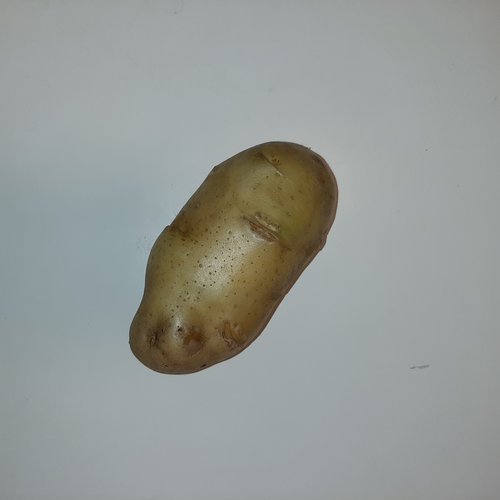
\includegraphics[width=\textwidth]{Imagen_original_20241128_174112.png}  % Cambia la ruta a la imagen
        \caption{Imagen original\textit{}}
    \end{minipage}\hfill
    % Imagen 2
    \begin{minipage}{0.43\textwidth}
        \centering
        \includegraphics[width=\textwidth]{Imagen_después_del_filtro-_gaussian_20241128_174115.png}  % Cambia la ruta a la imagen
        \caption{Imagen luego de aplicar gaussian blur}
    \end{minipage}
\end{figure}
   
 Debe notarse como prácticamente la imagen queda igual, esto es por la alta resolución de la misma, aun así el filtro gaussiano limpia exitosamente el ruido de fondo.
\begin{figure}[htbp]
    \centering
    % Imagen 1
    \begin{minipage}{0.43\textwidth}
        \centering
        \includegraphics[width=\textwidth]{Imagen_después_del_filtro-_binarizedADAPTIVE_20241128_175600.png}  % Cambia la ruta a la imagen
        \caption{Imagen binarizada sin filtrado previo}
    \end{minipage}\hfill
    % Imagen 2
    \begin{minipage}{0.43\textwidth}
        \centering
        \includegraphics[width=\textwidth]{Imagen_después_del_filtro-_morfologico_20241128_175610.png}  % Cambia la ruta a la imagen
        \caption{Filtro morfológico sin filtrado previo}
    \end{minipage}
    \centering
    % Imagen 1
    \begin{minipage}{0.43\textwidth}
        \centering
        \includegraphics[width=\textwidth]{Imagen_después_del_filtro-_binarizedADAPTIVE_20241128_174117.png}  % Cambia la ruta a la imagen
        \caption{Imagen binarizada con blur aplicado}
    \end{minipage}\hfill
    % Imagen 2
    \begin{minipage}{0.43\textwidth}
        \centering
        \includegraphics[width=\textwidth]{Imagen_después_del_filtro-_morfologico_20241128_174118.png}  % Cambia la ruta a la imagen
        \caption{Filtro morfológico con blur aplicado}
    \end{minipage}
\end{figure}
\newpage
\subsubsection*{Extracción de características}

Una vez que se han aplicado los filtros, se procede con la extracción de características de la imagen procesada. En esta sección se detallan los pasos utilizados para obtener las características.

\begin{itemize}
    \item \textbf{Detección de contornos}
    \begin{itemize}
        \item \textbf{Descripción:} Se identifican los contornos en la imagen utilizando el algoritmo \texttt{cv2.findContours}. Este proceso permite detectar las fronteras de los objetos presentes en la imagen.
        \item \textbf{Parámetros:}
        \begin{itemize}
            \item \texttt{cv2.RETR\_EXTERNAL}: Modo de recuperación de contornos que solo extrae los contornos externos de los objetos.
            \item \texttt{cv2.CHAIN\_APPROX\_SIMPLE}: Método de aproximación de contornos que almacena solo los puntos extremos de los segmentos de contorno.
        \end{itemize}
        \item \textbf{Proceso:} 
        \begin{itemize}
            \item Se detectan los contornos presentes en la imagen procesada.
            \item Se selecciona el contorno con el área más grande, que generalmente representa el objeto de interés en la imagen.
        \end{itemize}
    \end{itemize}
\begin{figure}[h]
    \centering
    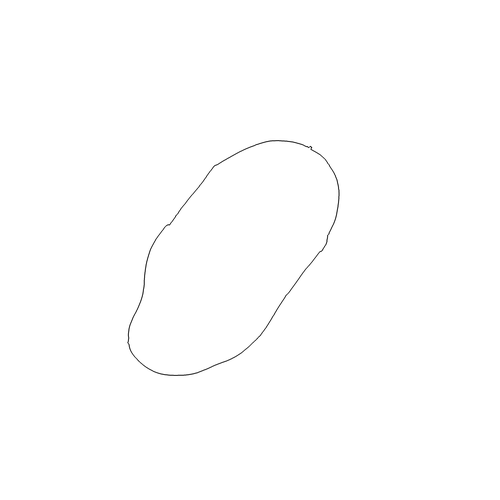
\includegraphics[width=0.5\linewidth]{Imagen_con_contornos_20241129_095157.png}
    \caption{Contorno capturado}
    \label{fig:enter-label}
\end{figure}
    \item \textbf{Cálculo de momentos de Hu}
    \begin{itemize}
        \item \textbf{Descripción:} Los momentos de Hu [\cite{wikipedia_image_moment} son invariantes a transformaciones geométricas (traslación, rotación y escala). Se utilizan para describir la forma del contorno y se calculan a partir del contorno más grande detectado.
        \item \textbf{Proceso:} 
        \begin{itemize}
            \item Se calculan el segundo y el tercer momento de Hu utilizando \texttt{cv2.moments} y \texttt{cv2.HuMoments}.
        \end{itemize}
    \end{itemize}

    \item \textbf{Cálculo del color promedio}
    \begin{itemize}
        \item \textbf{Descripción:} El color promedio dentro del área delimitada por el contorno detectado se calcula como una característica adicional.
        \item \textbf{Proceso:} 
        \begin{itemize}
            \item Se utiliza una máscara generada a partir del contorno para extraer los píxeles dentro de la región de interés.
            \item Se aumenta la saturación y el brillo de la imagen dentro de la mascara con factores de 1.03 y 1.7 respectivamente.
            \item Se calcula el valor promedio de los canales de color (Rojo, Verde, Azul) de los píxeles en esa región.
        \end{itemize}
    \end{itemize}

    \item \textbf{Almacenamiento y visualización de características}
    \begin{itemize}
        \item \textbf{Descripción:} Los momentos de Hu y el color promedio se guardan en un archivo CSV para su posterior análisis o clasificación.
        \item \textbf{Proceso:} 
        \begin{itemize}
            \item Los momentos de Hu seleccionados y el color promedio se almacenan en un archivo de tipo CSV con encabezados apropiados.
            \item Se visualiza la imagen procesada, destacando los contornos y mostrando la región de interés.
        \end{itemize}
\end{itemize}
\end{itemize}


\subsubsection*{Dimensionalidad y PCA}
    Para el caso de las imágenes las dimensiones iniciales son 5, dado que se tienen:
\begin{itemize}
    \item 3er Momento de Hu
    \item 4to Momento de Hu
    \item Media del color Rojo
    \item Media del color Verde
    \item Media del color Azul
\end{itemize}
    Es importante aclarar que de forma matemática el algoritmo KMeans utiliza la distancia Euclidiana para la clusterización, la misma pierde sentido en más de 3 dimensiones, pero, aun así funciona de forma aceptable dado que solo se esta excediendo por 2 la dimensionalidad recomendada. De todas maneras, se experimento con dos métodos de reducción de dimensionalidad, el primero, PCA \ref{fig:pca_img} muestra una separación aunque aceptable, no suficiente para el algoritmo dado que se pretende trabajar con una dimensionalidad reducida, luego se encuentra UMAP \ref{fig:umap_img} que muestra una notable separación de los datos, obteniendo ventajas en la clusterización por KMeans y en la eficiencia del modelo.
    
\begin{figure}[htbp]
    \centering
    % Imagen 1
    \begin{minipage}{0.8\textwidth}
        \centering
            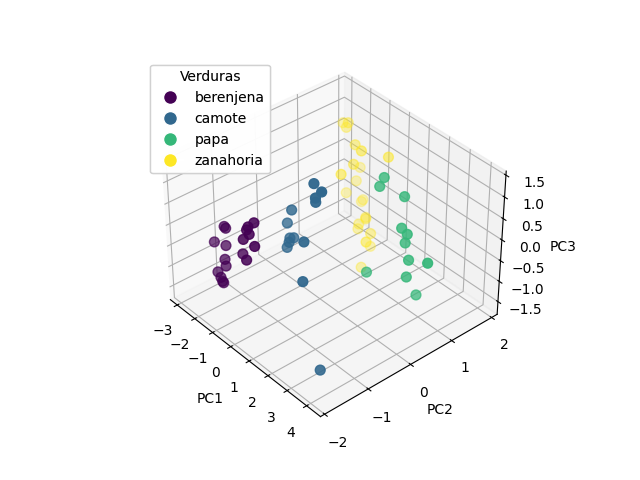
\includegraphics[width=0.85\linewidth]{Figure_1.png}
            \caption{PCA (3 componentes) realizado a las 5 componentes iniciales}
            \label{fig:pca_img}
    \end{minipage}\hfill
    % Imagen 2
    \begin{minipage}{0.8\textwidth}
         \centering
    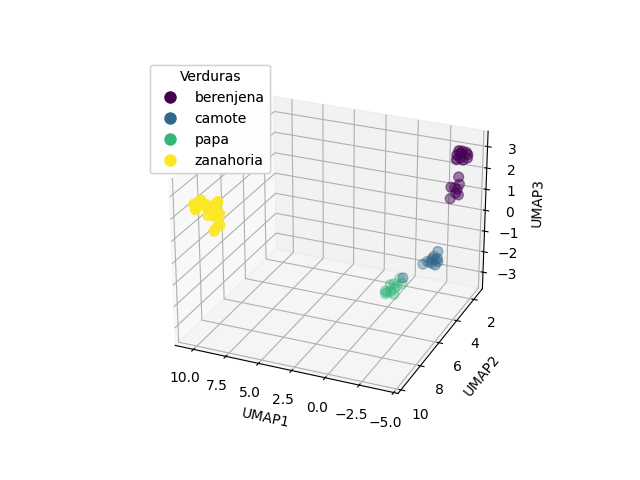
\includegraphics[width=0.85\linewidth]{umap_imagenes.png}
    \caption{UMAP (3 componentes) realizado a las 5 componentes iniciales}
    \label{fig:umap_img}
    \end{minipage}
\end{figure}
\subsection{Clasificador de audios}
En el caso del clasificador de audios, al tratarse de una agente que aprende de forma supervisada, la cátedra consigna el uso del conocido algoritmo KNN. \newline
Se eligió la particularidad de utilizar siempre un valor de K impar, para no resolver innecesarios empates.\newline
Para el calculo de la distancia se utiliza la distancia de Minkowski con un valor de p igual a 2, dando como resultado la distancia Euclidiana en n-dimensiones.\newline
La distancia de Minkowski entre dos puntos \( x = (x_1, x_2, \dots, x_n) \) y \( y = (y_1, y_2, \dots, y_n) \) en un espacio \( n \)-dimensional es:

\[
d(x, y) = \left( \sum_{i=1}^{n} |x_i - y_i|^p \right)^{\frac{1}{p}}
\]
\begin{algorithm}
\caption{Algoritmo de K-Nearest Neighbors (KNN)}
\begin{algorithmic}[1]
\Require $X = \{x_1, x_2, \dots, x_n\}$: conjunto de entrenamiento con $n$ ejemplos.\\
\Require $Y = \{y_1, y_2, \dots, y_n\}$: etiquetas correspondientes al conjunto de entrenamiento.\\
\Require $k$: número de vecinos más cercanos a considerar.\\
\Require $x_{\text{query}}$: ejemplo de consulta (punto de datos para clasificar).
\Ensure Predicción de clase para $x_{\text{query}}$.

\State \textbf{Paso 1:} Calcular la distancia entre $x_{\text{query}}$ y cada punto de entrenamiento $x_i$.\\
\State \textbf{Paso 2:} Ordenar los puntos de entrenamiento en función de las distancias calculadas.\\
\State \textbf{Paso 3:} Seleccionar los $k$ vecinos más cercanos.\\
\State \textbf{Paso 4:} Obtener las etiquetas de los $k$ vecinos seleccionados: $y_1, y_2, \dots, y_k$.\\
\State \textbf{Paso 5:} Realizar una votación para determinar la clase mayoritaria entre las etiquetas $y_1, y_2, \dots, y_k$.\\
\State \textbf{Paso 6:} Devolver la clase mayoritaria como la predicción para $x_{\text{query}}$.
\end{algorithmic}
\end{algorithm}
\newpage
\subsubsection*{Estrategia de base de datos}
Para el caso de la base de datos de los audios se opto por un enfoque inclinado a tener una gran cantidad de datos (alrededor de 380 muestras), la justificación  para esto es el hecho de que la idea inicial era que no se limitara a ciertas voces, ya sea por el timbre de la voz dado el sexo o cualquier otra característica adicional, en pocas palabras una gran base de datos implica robustez ya que, al fin y al cabo, el modelo se entrena con mas ruido y es mas propenso a 'aprender' patrones, aunque también implica un gran costo computacional para el procesamiento de las muestras.

\subsubsection*{Preprocesamiento del audio}
En este proyecto, el audio pasa por una serie de etapas de preprocesamiento antes de ser utilizado para la clasificación de palabras. A continuación se describen los pasos seguidos en el filtrado y la normalización del audio:

\begin{itemize}

\item \textbf{Pre-énfasis:}
  \begin{itemize}
    \item La etapa de pre-énfasis tiene como objetivo resaltar las altas frecuencias del audio para mejorar la discriminación de las características. Esto es particularmente útil en el procesamiento de señales de voz, ya que ayuda a compensar la atenuación de frecuencias altas en el canal de transmisión. 
    \item Se aplica un filtro de pre-énfasis con un coeficiente de 0.99 usando la función \texttt{preemphasis} de \texttt{librosa} \footnote{Mas detalles en \cite{librosa}}. Esto amplifica las frecuencias altas y prepara el audio para las siguientes etapas de filtrado.
  \end{itemize}

\item \textbf{Filtro paso banda dinámico:}
  \begin{itemize}
    \item El audio pasa por un filtro paso banda dinámico para eliminar las frecuencias fuera de un rango útil para la clasificación de las palabras. Este filtro ayuda a reducir el ruido en frecuencias no relevantes para la tarea de clasificación y mejora la calidad de las características extraídas.
    \item Se configura un filtro de Butterworth de orden 4, con un corte bajo en 50 Hz y un corte alto en 8000 Hz. El corte superior se ajusta dinámicamente para no superar la frecuencia de Nyquist, que depende de la tasa de muestreo \(sr\) del audio.
    \item El filtro se aplica usando la función \texttt{signal.butter} para crear los coeficientes del filtro y \texttt{signal.filtfilt} para aplicar el filtro al audio pre-énfasis. Este paso elimina frecuencias no deseadas, especialmente por debajo de 50 Hz y por encima de 8000 Hz.
  \end{itemize}
\newpage
\item \textbf{Reducción de ruido:}
  \begin{itemize}
    \item La reducción de ruido se lleva a cabo utilizando un enfoque basado en la descomposición de la transformada de Fourier (STFT) y un umbral de ruido adaptativo. Este paso permite eliminar componentes no deseadas del audio que corresponden a ruido ambiental o interferencias.
    \item Primero, se calcula la STFT del audio filtrado y se obtiene el espectro de magnitudes \(S\). Se calcula un umbral de ruido basado en la media del espectro, multiplicado por un factor de 1.5. Luego, se aplica una máscara para reducir las componentes espectrales que están por debajo de este umbral.
    \item Esta máscara se ajusta mediante el uso de un filtro de vecindad mediana para refinar la estimación de las componentes útiles. La fase se mantiene intacta y se reconstruye la señal limpia mediante la inversa de la STFT (\texttt{istft}).
  \end{itemize}

\item \textbf{Normalización de Loudness:}
  \begin{itemize}
    \item La normalización de la loudness (volumen percibido) se realiza para garantizar que el nivel de volumen del audio esté dentro de un rango objetivo estándar. Esto es especialmente importante en tareas de clasificación, ya que los modelos pueden verse afectados por variaciones en el volumen de las grabaciones.
    \item Se utiliza el medidor de loudness de \texttt{pyln.Meter} para calcular el \texttt{loudness\_actual} del audio filtrado. Luego, se ajusta el volumen del audio para que el nivel de loudness coincida con un valor objetivo de -23 LUFS (Loudness Units Full Scale), que es el estándar para audio de calidad.
    \item La función \texttt{pyln.normalize.loudness} ajusta la loudness del audio, asegurando que el volumen final sea adecuado para su posterior procesamiento y clasificación.
  \end{itemize}

\end{itemize}
\subsubsection*{Extracción de caracteristicas}
Se extraen varias características acústicas del audio para su clasificación. Estas características se calculan tanto para cada segmento del audio como para el archivo de audio completo. Es importante aclarar que la extracción de estas se realiza mediante la conocida libreria para tratamiento de señales \texttt{librosa}, disponible para Python.

\begin{itemize}

\item \textbf{13 MFCCs (Mel-Frequency Cepstral Coefficients):}
  \begin{itemize}
    \item Para cada segmento del audio, se calculan los 13 coeficientes \texttt{MFCC}, que representan las características espectrales más importantes de la señal. La media de cada uno de los 13 coeficientes se calcula a lo largo de todo el segmento, lo que proporciona una descripción compacta y estable de las características acústicas de la palabra en ese segmento. 
    \item Estos coeficientes son cruciales para capturar las variaciones espectrales que permiten diferenciar las 4 palabras. Cada palabra tiene un patrón acústico único que puede ser descrito por sus coeficientes MFCC. Al calcular la media, se obtienen representaciones robustas de cómo las características espectrales de la palabra se comportan en el tiempo.
  \end{itemize}

\item \textbf{Estadísticas adicionales de los 13 MFCCs:}
  \begin{itemize}
    \item Además de la media, se calculan tres estadísticas adicionales para cada uno de los 13 coeficientes MFCC:
      \begin{itemize}
        \item \textbf{Valor máximo:} El valor máximo de cada uno de los coeficientes MFCC proporciona información sobre los picos espectrales dentro del segmento de audio. Las palabras pueden tener características distintivas que se manifiestan como picos espectrales en ciertas frecuencias, y capturar estos máximos puede ser útil para diferenciarlas.
        \item \textbf{Valor mínimo:} El valor mínimo de los coeficientes MFCC resalta las frecuencias menos prominentes de la palabra, lo que puede ayudar a identificar las partes de la palabra que tienen una presencia espectral más baja o sutil, y también a distinguir entre palabras con un patrón espectral menos intenso.
        \item \textbf{Desviación estándar:} La desviación estándar captura la variabilidad de los coeficientes MFCC dentro del segmento. Una baja desviación estándar indica una señal más constante, mientras que una alta desviación estándar puede indicar una mayor variabilidad en las características espectrales, lo cual es importante para distinguir palabras que tienen variabilidad en su pronunciación.
      \end{itemize}
  \end{itemize}

\item \textbf{RMS (Root Mean Square):}
  \begin{itemize}
    \item El valor \texttt{RMS} se calcula para cada segmento de audio y mide la amplitud promedio de la señal. Este valor es crucial para determinar la "intensidad" general de la señal. Las 4 palabras pueden tener diferentes niveles de intensidad acústica (por ejemplo, algunas pueden ser pronunciadas con más énfasis o mayor volumen). El cálculo del RMS ayuda a capturar esta variabilidad y es útil para identificar patrones relacionados con la pronunciación de las palabras.
  \end{itemize}

\item \textbf{Duración del Audio:}
  \begin{itemize}
    \item La \texttt{duración} del audio es una característica única que mide el tiempo total de la grabación, en segundos. En este caso, la duración es relevante porque las 4 palabras a clasificar tienen una duración aproximada consistente, y la duración total del archivo de audio puede ayudar a identificar patrones de tiempo que están asociados con las palabras específicas. Aunque no se calcula por segmento, la duración total de la grabación puede servir como una referencia útil para el modelo, especialmente si se tiene en cuenta la variabilidad de la duración de las palabras en diferentes entornos acústicos o de pronunciación.
  \end{itemize}

\end{itemize}
\subsubsection*{Tratamiento de dimensionalidad}
Este agente se caracteriza por tener que lidiar con un conjunto de datos de gran dimension a comparación del agente anterior, finalmente se obtiene un conjunto de datos de 209 dimensiones. La realidad es que aunque KNN podría llegar a funcionar aun teniendo tantas componentes, la probabilidad de encontrar vecinos \textbf{realmente cercanos} es cada vez menor. Se tratará en el apéndice más detalles sobre esto. 
Primero se propuso la utilización de PCA al igual que en el clasificador de imágenes, funcionando correctamente cuando se reducían las dimensiones a 15, esto reducía bastante el costo computacional pero aun así la separación de de los clusters no era del todo convincente. Por lo que mediante una serie de prompts a ChatGPT, se propuso la utilización de UMAP (Uniform Manifold Approximation and Projection) el cual logró una considerable separación de clusters a comparación de PCA, además de logrando reducir la dimensionalidad del problema a solo 3, por lo tanto, finalmente las distancias son realizadas en 3 dimensiones y el algoritmo no pierde su sentido geométrico.

\begin{figure}[htbp]
    \centering
    % Imagen 1
    \begin{minipage}{0.45\textwidth}
        \centering
        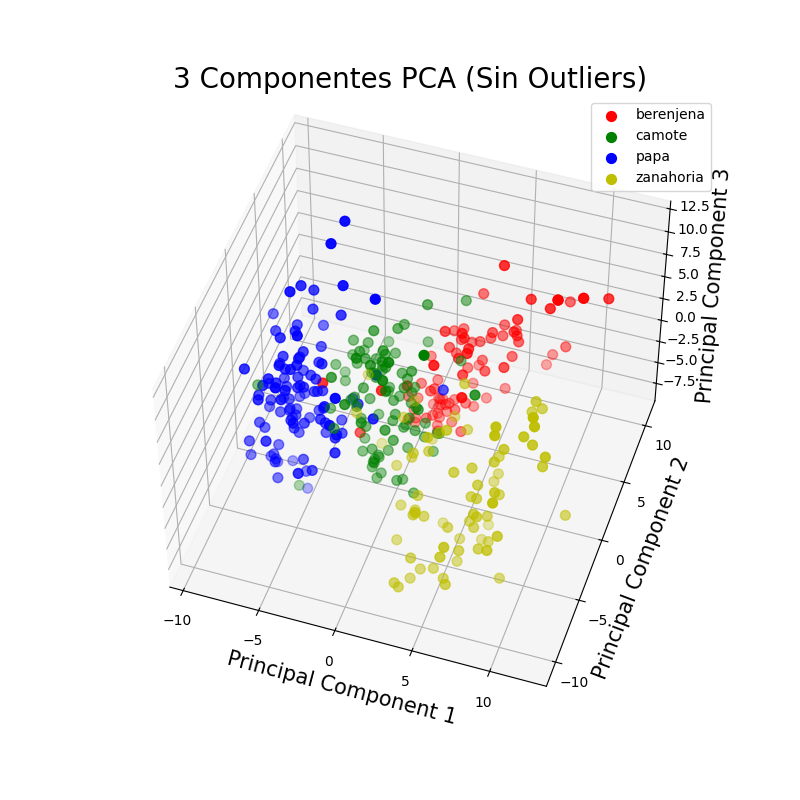
\includegraphics[width=\textwidth]{pca_audio.png}
        \caption{Datos luego de aplicar PCA en 3 dimensiones.}
        \label{fig:pca_audio}
    \end{minipage}
    \hfill
    % Imagen 2
    \begin{minipage}{0.45\textwidth}
        \centering
        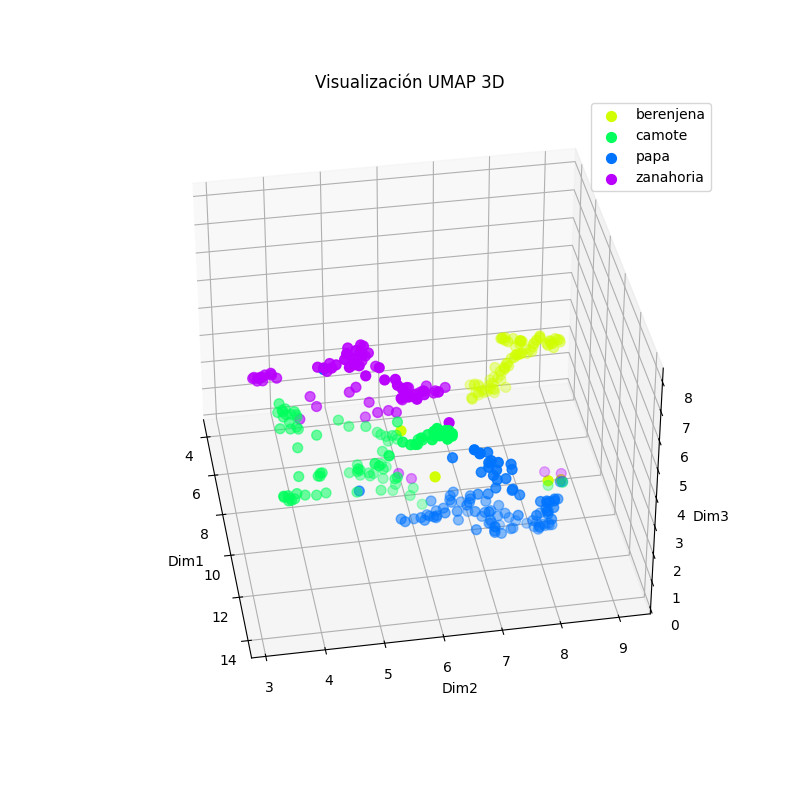
\includegraphics[width=\textwidth]{umap_audio.png}
        \caption{Datos luego de aplicar UMAP en 3 dimensiones.}
        \label{fig:umap_audio}
    \end{minipage}
    \caption{Comparación entre PCA y UMAP aplicados a los datos en 3 dimensiones.}
    \label{fig:comparacion_pca_umap}
\end{figure}

Es notable la filtración al ruido que realiza UMAP, aun así es importante destacar que aunque este algoritmo obtiene grandes resultados en terminos de redimensionalidad, no sería posible si el conjunto de datos inicial de n-dimensiones no formara subespacios, es decir que si la información original no respetara alguna relación UMAP no tiene la capacidad de generarla.
\newpage
\subsection{Eficiencia de los agentes}
Para el clasificador de audios la estrategia de comprobación de eficiencia fue la de a partir de la base de datos original, entrenar al algoritmo con un 70\% de la información, se utilizaba el 30\% restante para como muestras de prueba. Este enfoque no siempre presentaba resultados coherentes frente a la prueba de campo cuando un ser humano debía grabar una nueva voz y pasarla como muestra al sistema, aun así era un indicativo de si se estaba empeorando o no la estrategia de características.
Aun así a veces ya sea por overfitting o por la cantidad tan grande de datos que se tienen arrojaba eficiencias superiores al 90\% aun cuando el sistema mostraba grandes deficiencias en pruebas de campo. \newline Finalmente se termino obteniendo una eficiencia del 94\% que al menos si representa las pruebas de campo.

\section{Repositorio del proyecto}
Se adjunta el link al repositorio que contiene toda la información respecto al código fuente, y el códio fuente en si mismo. \newline 
\url{https://github.com/fcastel2002/Trabajo-final-IA1---Castel }

\newpage

%--- Section ---%
\section{Conclusiones}
Son varias las conclusiones extraídas del proyecto presentado, la primera es que para el clasificador de imágenes, existen bastantes limitantes al momento de diseñar un modelo robusto y a prueba de variaciones en el entorno, sobre todo por las particularidades del sensor que presenta el agente, al fin y al cabo extraer los colores de una verdura es un proceso que aunque eficiente si se realiza siempre en el mismo entorno, muy susceptible a variaciones de iluminación, por suerte los momentos de Hu impiden de cierta forma confundir notablemente dos verduras que tengan colores similares, así se presentarían enormes dificultades con el agente diseñado si se pretendiera realizar la clasificación de verduras con colores similares o directamente iguales. Por otro lado en el caso del clasificador de audio se obtuvieron conclusiones mucho más enriquecedoras, primero se tiene la muy notable influencia de los coeficientes cepstrales, los cuales diferencian sustancialmente a las palabras (es de esperarse dado que estos coeficientes se calculan en escala MEL, la misma escala para obtener los Espectogramas MEL [\ref{fig:mel_img}], estos son comunmente utilizados en la clasificación de audios con redes neuronales en formato imagen), luego fue interesante el descubrimiento de que la tasa de cruces por cero no estaba arrojando valores relevantes más bien estaba añadiendo ruido al conjunto de datos.
\begin{figure}[h]
    \centering
    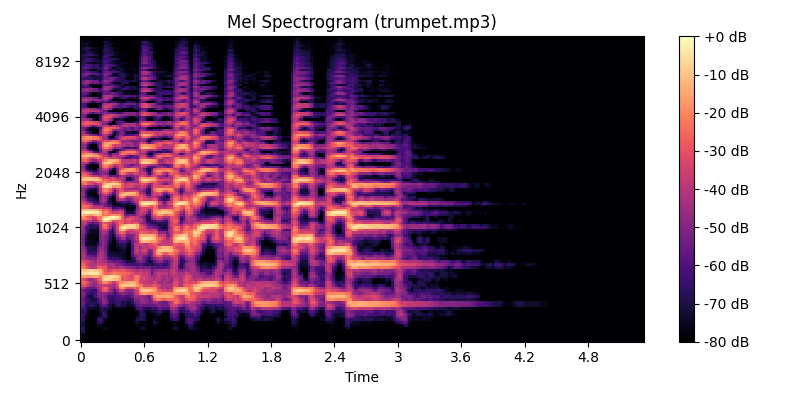
\includegraphics[width=0.75\linewidth]{mel_diagram.png}
    \caption{Imagen tomada de https://notesbylex.com/melspectrogram }
    \label{fig:mel_img}
\end{figure}
\subsection*{Generalización de los datos}
\subsubsection*{Clasificador de audios}
A mitad de proyecto se pretendió hacer más robusto el modelo mediante una normalización del tono a través la extracción de la frecuencia relacionada al mismo F0, para realizar una normalización en todos los audios, así, se lograría que el sistema de reconocimiento funcionara tanto como para voces graves como para voces agudas. Este enfoque trajo mas problemas que soluciones dado que el proceso de normalización de tono no es preciso y es complejo que los audios queden con el mismo tono. Finalmente se decidió por expandir enormemente la base de datos de aproximadamente 50 audios a 380. Además se llegó a la conclusión de que los coeficientes que se estaban extrayendo no eran sumamente dependientes del tono de los audios, por lo que tener audios de distinto tono no genero una dispersión notable.
\subsubsection*{Clasificador de imágenes}
Al principio se propuso utilizar los 7 Momentos de Hu, sin los colores promedios, lo que realmente no generaba ningún tipo de patrón distinguible en los datos, luego se implemento la obtención del color promedio pero esto no solucionaba lo anterior, llegando a la conclusión que la utilización de los 7 Momentos generaba ruido no despreciable en el conjunto de muestras, por lo que, realizando pruebas, se decidió quedarse solo con 2 Momentos de Hu, la realidad de las pruebas mostraba despreciable a la selección de momentos específicos, por lo tanto la elección de estos dos, es arbitraria.
\subsection*{Uso de IA generativa}
Para este proyecto se utilizaron dos principales IA generativas, la primera, ChatGPT, el cual fue de gran ayuda al momento de iniciar el proyecto y consultar sobre las características que se suelen extraer a las imágenes y a los audios, también sobre métodos de reducción de dimensionalidad, por otro lado proporcionó el código incial de los algoritmos, la segunda IA generativa que se utilizó fue Github Copilot, en su versión de Edits actualmente disponible para Visual Studio Code, la misma fue de suma ayuda al momento de realizar código, ya que en base a las propuestas de ChatGPT se realizaba el prompt correspondiente a Copilot, el cual conocía las librerías y los métodos de ellas. Los modelos LLM utilizados fueron GPT 4o, o1-mini y o1-preview para prompts que implicaban grandes modificaciones sobre todo en código.
\newline
Un claro ejemplo de un prompt que aumentó notablemente la eficiencia de los agentes fue a partir de mencionar que aunque la varianza de las características extraídas actualmente eran no correspondientes con características que son redundantes, y además también parecía mostrar cierta diferencia para cada etiqueta el diagrama de PCA no mostraba suficiente separación de las distintas etiquetas, este fue el precursor de que la IA generativa propusiera utilizar otras técnicas de re dimensionamiento de la información, como por ejemplo UMAP, esta implementación fue clave en el proyecto, además hizo que se dedicara extensamente a investigar en este área. 
\newline
Creo que para este proyecto el uso de este tipo de herramientas fue fundamental para comprender más que es lo que se estaba haciendo, al fin y al cabo la utilización de la misma depende de el uso que se le dé y la conciencia con la que se realice.
\newpage


%-------------------------------------------
% Optional Contents
%-------------------------------------------








%-------------------------------------------
% References
%-------------------------------------------

% Print bibliography
\nocite{*}
\printbibliography



%-------------------------------------------
% Appendix
%-------------------------------------------
% Activate the appendix in the doc
% from here on sections are numerated with capital letters 
%\appendix

\newpage


\appendix
\section*{Apéndice A: Reducción de Dimensionalidad con UMAP}

En este proyecto, se empleó la técnica de reducción de dimensionalidad UMAP (Proyección Uniforme Aproximada y Manifold) para transformar los datos originales a un espacio de menor dimensionalidad. Este paso fue esencial para mejorar la eficiencia computacional y facilitar la interpretación de los resultados en ambos agentes (no supervisado y supervisado).

La técnica PCA (Análisis de Componentes Principales) fue considerada inicialmente; sin embargo, debido a su naturaleza lineal, no logró filtrar adecuadamente el ruido presente en los datos, lo que motivó la elección de UMAP como una alternativa más robusta.

\subsection*{A.1 UMAP (Uniform Manifold Approximation and Projection)}
UMAP es una técnica de reducción de dimensionalidad no lineal que:
\begin{itemize}
    \item Conserva las relaciones locales entre los puntos de datos, asegurando que puntos cercanos en el espacio original permanezcan cercanos en el espacio reducido.
    \item Se basa en la teoría de grafos y manifolds para modelar relaciones complejas entre los puntos, siendo especialmente útil en conjuntos de datos con ruido o estructuras no lineales.
    \item Permite una reducción eficaz incluso en espacios de alta dimensionalidad, manteniendo patrones significativos en los datos.
\end{itemize}

\subsection*{A.2 Aplicación de UMAP en el Proyecto}
UMAP fue utilizado en ambos agentes para reducir la dimensionalidad, con los siguientes resultados:

\begin{itemize}
    \item \textbf{Agente No Supervisado:}
    \begin{itemize}
        \item Los datos originales tenían 5 dimensiones.
        \item UMAP redujo los datos a un espacio de 3 dimensiones, lo que permitió visualizar y explorar mejor los patrones intrínsecos de los datos no etiquetados.
        \item Este paso fue crucial para mejorar el rendimiento del agente, ya que las relaciones clave en los datos fueron destacadas mientras que el ruido fue minimizado.
    \end{itemize}

    \item \textbf{Agente Supervisado:}
    \begin{itemize}
        \item Los datos originales tenían 209 dimensiones, lo que representaba un desafío debido a la alta dimensionalidad y al ruido inherente.
        \item UMAP redujo estos datos a 3 dimensiones, conservando las relaciones relevantes para la tarea de clasificación supervisada.
        \item Esta reducción ayudó a evitar problemas relacionados con la "maldición de la dimensionalidad" y mejoró la eficiencia del modelo, tanto en el entrenamiento como en la predicción.
    \end{itemize}
\end{itemize}

\subsection*{A.3 Importancia de la Reducción de Dimensionalidad con UMAP}
La elección de UMAP como técnica de reducción de dimensionalidad fue crítica para el éxito de este proyecto debido a las siguientes ventajas:
\begin{itemize}
    \item \textbf{Manejo del ruido:} UMAP filtró eficazmente el ruido presente en los datos originales, algo que no se logró con PCA.
    \item \textbf{Eficiencia computacional:} Trabajar con datos reducidos a 3 dimensiones permitió una reducción significativa en el tiempo y los recursos computacionales necesarios para entrenar los modelos.
    \item \textbf{Mejora de la visualización:} La reducción a 3 dimensiones facilitó la interpretación de los patrones en los datos, especialmente en el agente no supervisado.
    \item \textbf{Preservación de relaciones relevantes:} UMAP conservó las estructuras locales y globales importantes en los datos, asegurando que las transformaciones no degradaran la calidad de la información.
\end{itemize}

\subsection*{A.4 Conclusión}
La implementación de UMAP fue determinante para este proyecto, permitiendo una reducción de dimensionalidad eficiente y efectiva en ambos agentes. Al reducir el espacio de 5 a 3 dimensiones para el agente no supervisado y de 209 a 3 dimensiones para el agente supervisado, se logró mejorar tanto la interpretabilidad como el rendimiento de los modelos, lo que demuestra la importancia de utilizar técnicas avanzadas de reducción de dimensionalidad en aplicaciones prácticas.

\end{document}

\end{document}